\section{Gradient}
\subsection{Problem Specification}

ABS-Normal Form:
\begin{flalign*}
\begin{pmatrix}
\Delta z \\
\Delta y
\end{pmatrix}
= 
\begin{pmatrix}
a \\
b
\end{pmatrix}
+
\begin{pmatrix}
Z & L \\
J & Y 
\end{pmatrix}
\circ
\begin{pmatrix}
\Delta x \\
|\Delta z |
\end{pmatrix}
\end{flalign*}

The problem here is to calculate the gradient of a PL function in abs-normal form. Given the following structures:
\begin{flalign*}
	a,b,Z,L,J,Y,m,n,s,\Delta z
\end{flalign*}
the gradient can be obtained in the following way:
\begin{flalign*}
	\Sigma = diag(sign(\Delta z))
\end{flalign*}
\begin{flalign*}
	\Delta z &= a + Z \Delta x + L \Sigma \Delta z \\
		     &= (I-L\Sigma)^{-1} (a+Z \Delta x) \\
	\Delta y &= b + J \Delta x + Y |\Delta z| \\
		     &= b + J \Delta x + Y \Sigma \big( (I-L\Sigma)^{-1} (a+Z \Delta x) \big) \\
		     &= b + Y \Sigma(I-L \Sigma)^{-1} a + \big( J + Y\Sigma(I-L\Sigma)^{-1}Z  \Big) \Delta x
\end{flalign*}
\begin{flalign}
	\gamma &= b + Y \Sigma(I-L \Sigma)^{-1} a \label{eq_gamma} \\
	\Gamma &= J + Y\Sigma(I-L\Sigma)^{-1}Z \label{eq_Gamma}
\end{flalign}
The gradient can now e calculated as:
\begin{flalign*}
	\Delta f(\Delta x) = \gamma + \Gamma \Delta x
\end{flalign*}

\subsection{Implementation}

For the implementation we heavily relied on CUBLAS routines. 
A simplified version of the core-function can be found in fig. \ref{fig_lst_grad}. The attentive reader might note that gridsize and blocksize are fixed for all the kernels in this function. We discuss our approach of choosing these parameters in section (..).

\begin{figure}
\begin{lstlisting}[language=cpp]
template <typename T>
void gradient(T *a, T *b, 
T *Z, T *L, 
T *J, T *Y,
T *dz,
T *Tss, T *I, T *K,
int m, int n, int s,
int gridsize, int blocksize,
T *gamma, T *Gamma)
//  d_Tss = diag(1) - L * diag(sign(dz))
initTss <<<gridsize, blocksize >>>(d_Tss,d_L, d_dz, s, s*s);
//  d_I = diag(1)
initIdentity <<<gridsize, blocksize >>> (d_I, s);
//  d_I = d_Tss * X	
getTriangularInverse(handle, d_Tss, d_I, s);
//	d_I = d_I * diag(sign(dz))
multWithDz <<<gridsize, blocksize >>>(d_I, d_dz, s);
//	d_K = d_Y * d_I
cublasDgemm(.,d_Y,.,d_I,d_K,));
//	d_gamma = d_b
//  d_Gamma = J
cudaMemcpy(d_gamma, d_b,.);
cudaMemcpy(d_Gamma, d_J,.);
//	d_gamma = d_gamma + K*a
cublasDgemv(.,d_K,., d_a,., d_gamma,.);
//  d_Gamma = d_Gamma + K*Z
cublasDgemm(.,d_K,d_Z,d_Gamma,m));
}
\end{lstlisting}
\label{fig_lst_grad}
\caption{Simplified Implementation of the gradient function}
\end{figure}

\subsection{Performance Experiments}
\subsubsection{Single Execution}
In this experiment we executed the gradient implementation on the GTX as well as on the Tesla and measured the data-upload time as well as the execution time of the function (fig. \ref{fig_grad_memory}).
\begin{figure}[ht]
	\centering
	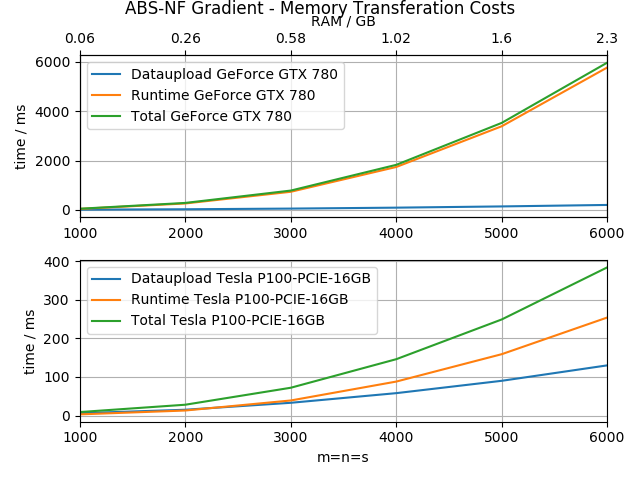
\includegraphics[width=0.6\textwidth]{img/gradient_memory.png}
	\caption{Multiple executions of the evaluate function on different devices}
	\label{fig_grad_memory}
\end{figure}
\subsubsection{Multiple  Executions}
In this experiment we measured the runtime of the serial version as well as the parallel version for a 100 executions of the gradient funciton. Data-transfer on and from the device was not included. The results can be found in fig. \ref{fig_grad_mult_executions}. Since the graphs are not quite detailed, we took some of the results into table (\ref{tab_grad_mult_executions}).
\begin{figure}[ht]
	\centering
	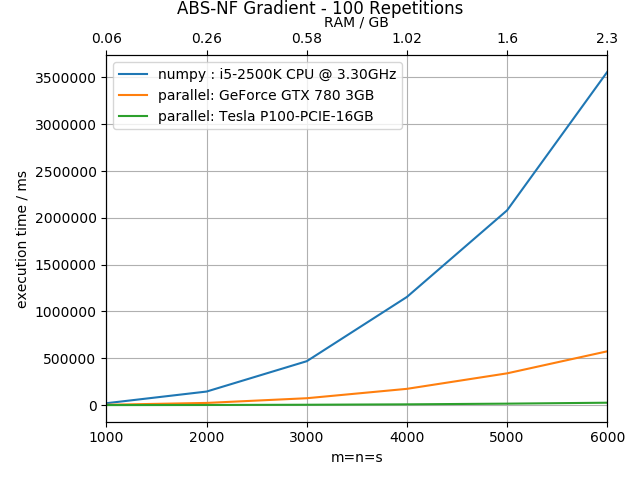
\includegraphics[width=0.6\textwidth]{img/gradient_mult_repetition.png}
	\caption{Multiple executions of the gradient function on different devices}
	\label{fig_grad_mult_executions}
\end{figure}
\begin{table}
	\centering
\begin{tabular}{c|c|c|c}
	$s=m=s$ & numpy (ms) & GTX (ms) & Tesla (ms) \\
	\hline
	1000 & 20008 & 3372 & 282 \\
	2000 & 144644 & 23122 & 1223 \\
	4000 & 1155222 & 173604 & 7947
	
\end{tabular}
\caption{This table shows some data}
\label{tab_grad_mult_executions}
\end{table}

Additionally we profiled a 100 executions of the gradient function with nvprof (table. \ref{tab_gradient_nvprof}).

\begin{table}
	\centering
	\begin{tabular}{c|c|c|c|c|c|l}
		Time(\%) &     Time  &   Calls  &      Avg  &      Min  &      Max  & Name \\
		\hline
		47.67\% &  11.8009s &      900 &  13.112ms &  358.57us &  90.166ms &  dgemm\_sm\_heavy\_ldg\_nn \\
		32.04\% &  7.93153s &      100 &  79.315ms &  77.982ms &  93.386ms &  dgemm\_sm\_heavy\_ldg\_nt \\
		5.77\% &  1.42887s &      900 &  1.5876ms &  95.107us &  10.248ms &  dgemm\_sm35\_ldg\_nn\_128x8x64x16x16 \\
		4.24\% &  1.05012s &      800 &  1.3126ms &  397.74us &  1.7257ms &  void kernel\_trsm\_l\_mul32 \\
		3.37\% &  835.25ms &      200 &  4.1763ms &  142.89us &  9.6000ms &  dgemm\_sm35\_ldg\_nn\_64x8x128x8x32 \\
		3.32\% &  820.79ms &      100 &  8.2079ms &  6.1753ms &  9.5876ms &  dgemm\_sm35\_ldg\_nt\_128x8x64x16x16 \\
		3.26\% &  806.34ms &      100 &  8.0634ms &  6.1730ms &  8.6610ms &  dgemm\_sm35\_ldg\_nt\_64x8x128x8x32 \\
		0.12\% &  29.230ms &      200 &  146.15us &  1.8560us &  294.63us &  [CUDA memcpy DtoD] \\
		0.09\% &  22.342ms &        8 &  2.7927ms &  1.1850us &  5.7200ms &  [CUDA memcpy HtoD] \\
		0.06\% &  15.472ms &      100 &  154.72us &  152.81us &  165.99us &  void gemv2N\_kernel\_val \\
		0.06\% &  13.796ms &      200 &  68.981us &  18.880us &  136.90us &  void trsm\_left\_kernel \\
		0.00\% &  1.1163ms &      100 &  11.162us &  10.848us &  14.016us &  void absnf::initTss \\
		0.00\% &  1.0580ms &      100 &  10.579us &  10.304us &  12.320us &  void absnf::multWithDz \\
		0.00\% &  557.88us &      100 &  5.5780us &  5.4400us &  7.3600us &  void absnf::initIdentity \\
	\end{tabular}
	\caption{Results of nvprof on the gradient function with 100 executions \label{tab_gradient_nvprof}}
\end{table}

\subsection{Analysis}
In contrast to the evaluate function, the parallel cuda version of the gradient function was magnitudes faster than the serial numpy version fig. (\ref{fig_grad_mult_executions}). It is important to note, that the numpy version is not optimized but rather a quick and dirty implementation to establish a baseline and should therefore not be considered as fastest serial approach.  \\
We can also see that the Tesla device here operates much faster than the GTX which can be deduced to the better double precision support. \\

In figure \ref{fig_grad_memory} a much better data-transfer to runtime ratio for both the GTX, as well as the Tesla are perceptible. This is important, since a batched version for data structures of size bigger than the global gpu memory may be worthwhile. \\

The profile in table  \ref{tab_gradient_nvprof} shows, that the majority of the runtime goes into the calculation of matrix-matrix products. The handcrafted kernels "initTss", "multWithDz" and "initIdentity" do not preponderate, as initially feared.